\documentclass{article}
\usepackage[T1]{fontenc}
\usepackage{lmodern}
\usepackage{graphicx}
\usepackage{amsmath,amssymb}
\usepackage[a4paper,margin=2cm]{geometry}
\usepackage[absolute,overlay]{textpos}
\setlength{\TPHorizModule}{1mm}
\setlength{\TPVertModule}{1mm}
\usepackage[indonesian]{babel}
\usepackage{hyperref}
\setlength{\emergencystretch}{2em}
% unit: Halaman 30

\begin{document}

% === Halaman 30 (llm) ===

P=Plaintext; C=Ciphertext; $K_x \approx$ P-array-entry $x$

\vspace{142.56mm}

$\oplus$ = xor

$\boxplus$ = addition mod $2^{32}$

% deskripsi: Diagram alur algoritma enkripsi blok yang menunjukkan struktur Feistel network dengan satu ronde yang terdiri dari F-Function (S-box 0-3), proses swap, pengulangan 15 ronde tambahan, pembatalan swap terakhir, dan output whitening menggunakan kunci K17 dan K18.
% bbox normalisasi: [0.2100, 0.3600, 0.7500, 0.8400]
\begin{textblock*}{113.40mm}(44.10mm,106.92mm)
\noindent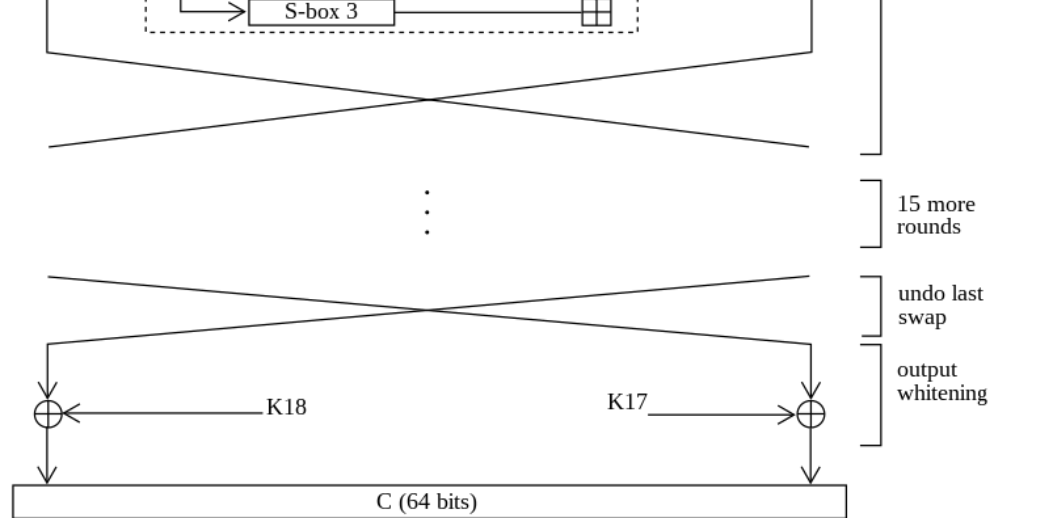
\includegraphics[width=113.40mm,height=142.56mm]{../../images/llm/page_030_img_01.png}%
\end{textblock*}

\end{document}
